% 对偶空间：对偶范数。

\section{对偶范数}
\label{sec:ls-dual-norms}

第~\ref{sec:ls-dual-spaces}节的线性泛函是对向量的读取。有了范数，就可以衡量一个读取有多大。误差分析中的典型问题是：误差$\bm r$只知道落在某个范数球内，一次加权读取$\bm z^\top\bm r$最多变化多少。在$\mathbb R^d$上取定一种范数后，这个最大值就是对偶范数。
\begin{definition}[对偶范数]
\label{def:linear-algebra-dual-norm}
给定$\mathbb R^d$上的范数，相对于标准坐标配对的\term{对偶范数}（dual norm）为
\begin{equation}
 \lVert\bm z\rVert_*=\sup_{\lVert\bm r\rVert\leq1}|\bm z^\top\bm r|.
 \label{eq:linear-algebra-dual-norm-definition}
\end{equation}
\end{definition}
这就是第~\ref{sec:ls-matrix-norms}节的诱导范数取输出空间为$\mathbb R$的情形：读取$\bm r\mapsto\bm z^\top\bm r$是$1\times d$矩阵$\bm z^\top$的作用。所以对任意范数，上确界有限并且可以取到。

对偶范数满足范数的各条要求，因而是对偶空间上的范数。非负性显然。$\bm z\neq\bm0$时，取$\bm z$的某个非零坐标$z_j$，则$\bm r=\bm e_j/\lVert\bm e_j\rVert$给出$|\bm z^\top\bm r|=|z_j|/\lVert\bm e_j\rVert>0$，这给出正定性。对每个$\bm r$都有$|(\bm z+\bm w)^\top\bm r|\leq|\bm z^\top\bm r|+|\bm w^\top\bm r|$，取上确界即得三角不等式；齐次性由$|(c\bm z)^\top\bm r|=|c|\,|\bm z^\top\bm r|$得到。图~\ref{fig:ls-dual-norm-unit-ball}把这个最大值画成支撑线最后接触单位球的位置。

\begin{figure}[!htb]
  \centering
  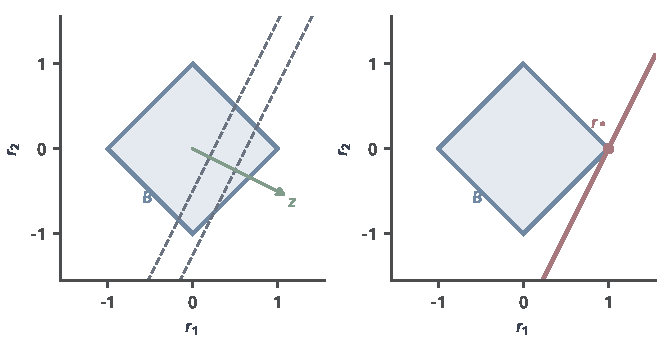
\includegraphics[width=112mm]{figures/00-shared/mathematical-preliminaries-upper/02-linear-spaces/matplotlib/ls-dual-norm-unit-ball/ls-dual-norm-unit-ball.pdf}
  \caption{对偶范数的几何：在原范数单位球$\lVert\bm r\rVert\leq1$上求线性读取$\bm z^\top\bm r$的最大值。左：原单位球（灰色）与读取方向$\bm z$；右：支撑直线最后接触单位球处给出$\lVert\bm z\rVert_*=\max_{\lVert\bm r\rVert\leq1}|\bm z^\top\bm r|$。对偶单位球（虚线）与原单位球互为极体。解析教学例。}
  \label{fig:ls-dual-norm-unit-ball}
\end{figure}

对$\ell_p$范数，对偶范数可以明确写出：
\begin{equation}
(\lVert\cdot\rVert_p)_*=\lVert\cdot\rVert_q,\qquad\frac1p+\frac1q=1.
\label{eq:linear-algebra-lp-duality}
\end{equation}
由齐次性，对任意预算$\rho\geq0$还有
\begin{equation}
 \max_{\lVert\bm r\rVert_p\leq\rho}|\bm z^\top\bm r|
 =\rho\lVert\bm z\rVert_q.
 \label{eq:linear-algebra-linear-perturbation-duality}
\end{equation}
Hölder不等式（定理~\ref{thm:linear-algebra-holder}）给出$\ell_p$单位球上的上界$\lVert\bm z\rVert_q$。这个上界可以达到。$1<p<\infty$且$\bm z\neq\bm0$时，取$r_j=|z_j|^{q-1}\operatorname{sgn}(z_j)/\lVert\bm z\rVert_q^{q-1}$；$\bm z=\bm0$时上界为零，任取可行输入即可。$p=1$时，把单位预算全部放在$|z_j|$最大的坐标上；$p=\infty$时，逐坐标取$r_j=\operatorname{sgn}(z_j)$。下面固定一个读取，比较三种误差预算。
\begin{example}[同一读取在三种误差预算下的最大变化]
\label{ex:ls-dual-norm-three-budgets}
取读取方向$\bm z=(2,-1)^\top$，即读取$\bm z^\top\bm r=2r_1-r_2$，让误差$\bm r$分别落在三种单位球内。

在$\ell_1$单位球上，预算只能分给各坐标的绝对值，全部放在权重$|z_j|$最大的第一个坐标最划算：$\bm r=(1,0)^\top$给出最大值$\lVert\bm z\rVert_\infty=2$。在$\ell_2$单位球上，最坏误差与$\bm z$同方向，取$\bm r=\bm z/\lVert\bm z\rVert_2=(2,-1)^\top/\sqrt5$，最大值为$\lVert\bm z\rVert_2=\sqrt5$。在$\ell_\infty$单位球上，每个坐标都可以同时取满，只需让符号与$z_j$一致：$\bm r=(1,-1)^\top$给出最大值$\lVert\bm z\rVert_1=3$。换成实际的误差预算$|r_j|\leq0.01$，就在式~\eqref{eq:linear-algebra-linear-perturbation-duality}中取$p=\infty$、$\rho=0.01$，最大变化为$0.01\cdot(2+1)=0.03$，由$\bm r=(0.01,-0.01)^\top$达到。

三种单位球给出的最大值依次为$2$、$\sqrt5$、$3$。读取本身没有变，变的是允许误差的形状：它决定了最坏方向在哪里，也决定了读取方向要用哪个对偶范数计量。
\end{example}
图~\ref{fig:linear-algebra-dual-unit-balls}画出这三种情形下的最坏方向。
\begin{figure*}[htbp]
  \centering
  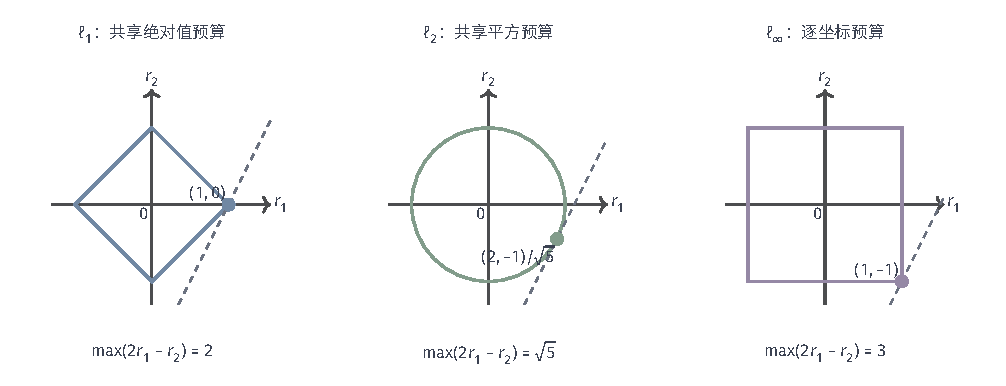
\includegraphics[width=168.998mm]{figures/00-shared/mathematical-preliminaries-upper/02-linear-spaces/tikz/linear-algebra-dual-unit-balls/figure.pdf}
  \caption{同一线性读取$2r_1-r_2$在$\ell_1$、$\ell_2$、$\ell_\infty$单位球上的最大值依次为$2$、$\sqrt5$、$3$。虚线为最后接触可行集的支撑直线，点为最大化方向。三图坐标尺度相同，均为解析教学例；允许误差的形状改变时，误差常数也随之改变。}
  \label{fig:linear-algebra-dual-unit-balls}
\end{figure*}

由此可见，误差预算按$\ell_\infty$给出时，读取方向要按$\ell_1$计量；预算按$\ell_2$给出时，读取方向仍按$\ell_2$计量。

原空间的范数改变，对偶范数随之改变。对加权的坐标范数，可以用换元把问题化回已知情形。
\begin{example}[加权$\ell_1$范数的对偶范数]
\label{ex:ls-weighted-dual-norm}
设权重$w_1,\ldots,w_d>0$，在$\mathbb R^d$上取加权范数$\lVert\bm r\rVert_{\bm w}=\sum_jw_j|r_j|$。把权重吸收进变量，令$s_j=w_jr_j$，则$\lVert\bm r\rVert_{\bm w}=\lVert\bm s\rVert_1$，$\bm z^\top\bm r=\sum_j(z_j/w_j)s_j$。$\bm r$取遍$\lVert\bm r\rVert_{\bm w}\leq1$时，$\bm s$恰好取遍$\ell_1$单位球。由式~\eqref{eq:linear-algebra-lp-duality}中$p=1$的情形，
\[
 \lVert\bm z\rVert_*=\max_j\frac{|z_j|}{w_j}.
\]
仍取上例的$\bm z=(2,-1)^\top$。不加权，即$\bm w=(1,1)^\top$时，$\lVert\bm z\rVert_*=2$，由$\bm r=(1,0)^\top$取到，与上例的$\ell_1$情形一致；改用$\bm w=(4,1)^\top$时，$\lVert\bm z\rVert_*=\max\{1/2,1\}=1$，由$\bm r=(0,-1)^\top$取到。

读取$\bm z^\top\bm r$的代数表达没有变，它的大小却随原空间的范数改变。第一个坐标的权重变大后，同样的预算只允许它有更小的变化，最坏方向因而转到第二个坐标。
\end{example}
所以讨论“输入误差最多引起多大输出误差”时，必须先说清误差用哪种范数度量。内积诱导的范数下，对偶范数等于表示向量的长度，在第~\ref{sec:ls-riesz-representation}节证明。一般有限维空间$V$上的线性泛函$\varphi$同样定义$\lVert\varphi\rVert_*=\max_{\lVert\bm v\rVert\leq1}|\varphi(\bm v)|$，它是取$W=\mathbb R$时的算子范数。无限维空间中，并非每个线性泛函都连续，代数对偶与连续对偶需要区分，这同样属于无限维理论。
